\documentclass{article}
\usepackage[utf8]{inputenc}
\usepackage{amsfonts}
\usepackage{amsthm}
\usepackage{amsmath}
\usepackage{enumerate}
\usepackage{hyperref}
\usepackage{amssymb}

\usepackage{float}
\usepackage{graphicx}

\begin{filecontents}[overwrite]{notes_hash-based-signatures.bib}
@misc{cryptoeprint:2014/795,
      author = {Daniel J.  Bernstein and Daira Hopwood and Andreas Hülsing and Tanja Lange and Ruben Niederhagen and Louiza Papachristodoulou and Michael Schneider and Peter Schwabe and Zooko Wilcox-O'Hearn},
      title = {{SPHINCS}: practical stateless hash-based signatures},
      howpublished = {Cryptology {ePrint} Archive, Paper 2014/795},
      year = {2014},
      url = {https://eprint.iacr.org/2014/795}
}
@misc{rfc8391,
    series =    {Request for Comments},
    number =    8391,
    howpublished =  {RFC 8391},
    publisher = {RFC Editor},
    doi =       {10.17487/RFC8391},
    url =       {https://www.rfc-editor.org/info/rfc8391/},
    author =    {A. Huelsing and D. Butin and S. Gazdag and J. Rijneveld and A. Mohaisen},
    title =     {{XMSS: eXtended Merkle Signature Scheme}},
    pagetotal = 74,
    year =      2018,
    month =     may,
}
\end{filecontents}
\nocite{*}


\theoremstyle{definition}



\title{Notes on hash-based signatures}
\author{arnaucube}
\date{January 2026}

\begin{document}

\maketitle

\begin{abstract}
    Notes taken while studying hash-based signatures.

    Usually while reading books and papers I take handwritten notes in a notebook, this document contains some of them re-written to $LaTeX$.
\end{abstract}

\tableofcontents

\vspace{1.0cm}

\section{Preliminaries}
\subsection{Lamport signatures (1979)}
(OTS: One Time Signature scheme)

\paragraph{key gen}

sk:
$$((s_{0,0}, s_{0,1}), (s_{1,0}, s_{1,1}), (s_{2,0}, s_{2,1}), \ldots, (s_{255,0}, s_{255,1}))$$
where each $s_{i,j} \in \{0, 2^256 -1\}$.

pk:
$$((h(s_{0,0}), h(s_{0,1})), (h(s_{1,0}), h(s_{1,1})), (h(s_{2,0}), h(s_{2,1})), \ldots, (h(s_{255,0}), h(s_{255,1})))$$

\paragraph{sign}
hash the 256 bits of the msg: $(m_0, \ldots, m_{255})$

and the signature is
$$(s_{0, m_0}, s_{1, m_1}, s_{2, m_2}, \ldots, s_{255, m_{255}})$$

\paragraph{verify}
compare hashes of signature components to elements of the public key.

\vspace{0.5cm}
Sizes: 16 kB sk and pk, 8 kB signature.

\subsection{Adding Merkle Trees (1979)}
idea: put a binary hash tree on top of all pk's: leaves are the hashes of pks.

Public key: root of the tree (256 bits)

Signature: OTS plus the authentication path (merkle proofs)

\paragraph{some numbers}
Fix to $2^{32}$ signatures.
\begin{itemize}
    \item key gen: compute the tree: $2^{33} -1$ hashes
    \item pk size: 32 bytes
    \item sk: the seed for the one-time signature (OTS) secret keys: 32 bytes
    \item signature size: $\approx$ 25 kB:
	\begin{itemize}
	    \item 8 kB Lamport signature
	    \item 16 kB Lamport pk
	    \item 32 $\cdot$ 32 = 1024 B of authentication path (merkle proofs)
	    \item 4 B for the index of the leaf node
	\end{itemize}
\end{itemize}

Main issue: have to remember the state, to update the secret key after each signing.


\subsection{Goldreich's approach (1986)}

\begin{itemize}
    \item make the tree huge (eg. height h=256), such that one can pick leaves at random
    \item each node corresponds to an OTS key pair
    \item leaf nodes are used to sign messages
    \item all OTS secret keys are generated from a seed
\end{itemize}

Numbers
\begin{itemize}
    \item pk and sk are still small, 32 bytes
    \item key gen is fast (only generate root OTS key pair)
    \item signing requires 2h=512 OTS key generations and h=256 OTS signatures
    \item signature is very large, eg. with Lamport OTS:
	\begin{itemize}
	    \item 256 $\cdot$ 24 kB for Lamport signatures and pks
	    \item 256 $\cdot$ 32 B for authentication paths
	    \item 32 B for the index of the leaf node
	\end{itemize}
	total size: 6 MB
\end{itemize}


\subsection{WOTS+}
Winternitz One-Time Signature.

\paragraph{Chaining function} $c^i(x,r)$

input values: $x \in \{0,1\}^n$, iteration counter: $i \in \mathbb{N}$,

bitmasks: $r=(r_1, \ldots, r_j) \in \{0,1\}^{n \times j}$, where $j \geq i$.

\begin{itemize}
    \item if $i=0$, return $x$; ie. $c^0(x,r)=x$
    \item if $i>0$,
	$$c^i(x,r)=  F(c^{i-1}(x,r) \oplus r_i)$$
	(where $\oplus$ is the bitwise XOR)
\end{itemize}

\paragraph{key generation}

$$sk, pk \leftarrow WOTS.keygen(S,r)$$

input seed: $S \in \{0,1\}^n$

bitmask: $r \in \{0,1\}^{n \times (w-1)}$

compute sk:

($G_l$ is a pseudorandom generator)

$$sk=(sk_1, \ldots, sk_l) \leftarrow G_l(S)$$
ie. the $n$ bit seed is expanded to $l$ values of $n$ bits

$$pk = (pk_1, \ldots, pk_l) = (c^{w-1}(sk_1, r), \ldots, c^{w-1}(sk_l, r))$$

\paragraph{signature:} $\sigma \leftarrow~ WOTS.sign(M, S, r)$

for a message $M \in \{0.1\}^n$

compute a base-w representation of $M$:
$$M = (M_1, \ldots, M_l),~~ M_i \in \{0, \ldots, w-1\}$$

compute checksum:
$$C = \sum_{i=1}^{l_1} (w-1-M_i)$$
and its base $w$ representation
$$C=(C_1, \ldots, C_{l_2})$$

set $B=(b_1, \ldots, b_l)=M||C$ (concatenation)

obtain sk with $sk \leftarrow~ WOTS.keygen(S,r)$

signature:

$$\sigma = (\sigma_1, \ldots, \sigma_l) = (C^{b_1}(sk_1, r), \ldots, C^{b_l}(sk_l, r))$$

\paragraph{verification:} $pk' \leftarrow~ WOTS.vf(M, \sigma, r)$

compute $b_i$ for $1 \leq i \leq l$ as described above

return:
$$pk' = (pk_1', \ldots, pk_l')\\
=(C^{w-1-b_1}(\sigma_1, r_{\stackrel{b+1, w-1}{1}}), \ldots, C^{2-1-b_l}(\sigma_l, r_{\stackrel{b+1, w-1}{l}}))
$$

and check that $pk \stackrel{?}{=} pk'$.

\subsection{HORST}
\paragraph{parameters}

$k, t=2^\tau$, with $k\tau=m$ (length of the message signed).

in SPHINCS-256: $t=2^16,~ k=32$.

\paragraph{key generation:} $pk \leftarrow HORST.keygen(S, Q)$

input seed: $S \in \{0,1\}^n$

bitmasks: $Q \in \{0,1\}^{2n \times \log t}$

$$sk=(sk_1, \ldots, sk_t) \leftarrow G_t(S)$$

Leaves of the tree are computed as $L_i=F(sk_i)$ for $i \in [t-1]$, and the tree is constructed using bitmasks $Q$.

pk: root node of a binary tree of height $\log t$.


\paragraph{signature:} $(\sigma, pk) \leftarrow~ HORST.sign(M, S, Q)$

$M \in \{0,1\}^m,~ S \in \{0,1\}^n,~ Q \in \{0,1\}^{2n \times \log t}$

Let $M=(M_0, \ldots, M_{k-1})$ be the $k$ numbers obtained by splitting $M$ into $k$ strings of length $\log t$ bits each, and interpreting each as an unsigned integer.

Signature:
$$\sigma = (\underbrace{\sigma_0, \ldots, \sigma_{k-1}}_{\stackrel{\sigma_i=(sk_{M_i}, Auth_{M_i})}{\text{for}~ i\in [k-1]}}, \sigma_k)$$

$Auth_{M_i}$: lower $\tau - x$ elements of the authentication path of the corresponding leaf $(A_0, \ldots, A_{\tau-1-x})$

$\sigma_k$: all the $2^x$ nodes of the binary tree on level $\tau-x$, $(N_{0,\tau-x}, \ldots, N_{2^x -1, \tau-x})$.

\paragraph{verification:} $pk' \leftarrow~ HORST.vf(M, \\sigma, Q)$

first compute $M_i$ as described in the signature step.

Then, for $i \in [k-1], ~ y_i = \lfloor M_i / 2^{\tau}-x \rfloor$, it computes $N'_{y_i, \tau-x}$ using root computation with index $M_i,~ L_{M_i}F(\sigma_i^1),~ Auth_{M_i}=\sigma_i^2$.

Then check $\forall~ i \in [k-1]$:
$$N'_{y_i, \tau-x} \stackrel{?}{=} N_{y_i, \tau-x}$$

ie. computed nodes match those in $\sigma_k$.

If ok, use $\sigma_k$ to compute the root ($= ~ N_{0, h}$), and return the root as $pk'$.



\section{SPHINCS (2015)}

\subsection{High level view}

\begin{itemize}
    \item hyper-tree of total height $h$
    \item each tree has height $h/d$
    \item inside the tree, use Merkle approach
    \item between trees use Goldreich approach
    \item sign messages with a "few-time" signature scheme (FTS)
\end{itemize}

\paragraph{SPHINCS-256} (128 bits of security)
\begin{itemize}
    \item 12 trees of height 5 each
    \item use WOTS as one-time-signature (OTS) scheme
    \item use HORST (HORS with tree) as few-time signature (FTS) scheme
    \item fix $n=256$ as bitlength of hashes in WOTS and HORST
    \item fix $m=512$ as size of the message hash (Blake-512)
    \item use ChaCha12 as pseudorandom generation
\end{itemize}

\subsection{SPHINCS construction}
\subsubsection{Parameters}

Security parameter: $n \in \mathbb{N}$

Hash functions:
\begin{align*}
&F: \{0,1\}^n \longrightarrow \{0,1\}^n\\
&H: \{0,1\}^{2n} \longrightarrow \{0,1\}^n\\
&\mathcal{H}: \{0,1\}^n \times \{0,1\}^*  \longrightarrow \{0,1\}^m
\end{align*}

for $m=poly(n)$

Height of the hyper-tree: $h \in \mathbb{N}$ (and $h|d$):\\
\hspace*{2em}$d$ layers of trees, each of height $h/d$.


Each tree: leaves are $2^{h/d}$ L-Tree root nodes, that each is a pk of WOTS+.\\
\hspace*{2em}$\Longrightarrow$ a tree is a keypair that can be used to sign $2^{h/d}$ messages.


The hyper-tree has $d$ layers
\begin{itemize}
    \item on layer $d-1$ it has a single tree
    \item on layer $d-2$ it has $2^{h/d}$ trees
	\begin{itemize}
	    \item roots signed using WOTS+ key pairs of the tree on layer $d-1$
	\end{itemize}
\end{itemize}

In general: layer $i$: $2^{(d-1-i)(h/d)}$ trees, and the roots of these trees are signed using the WOTS+ key pairs of the trees on layer $i+1$.

Layer 0: each WOTS+ keypair is used to sign a HORST pk.

$\longrightarrow$ Full tree structure is never computed, values are determined by the seed and the bit masks.

\begin{figure}[H]
    \centering
    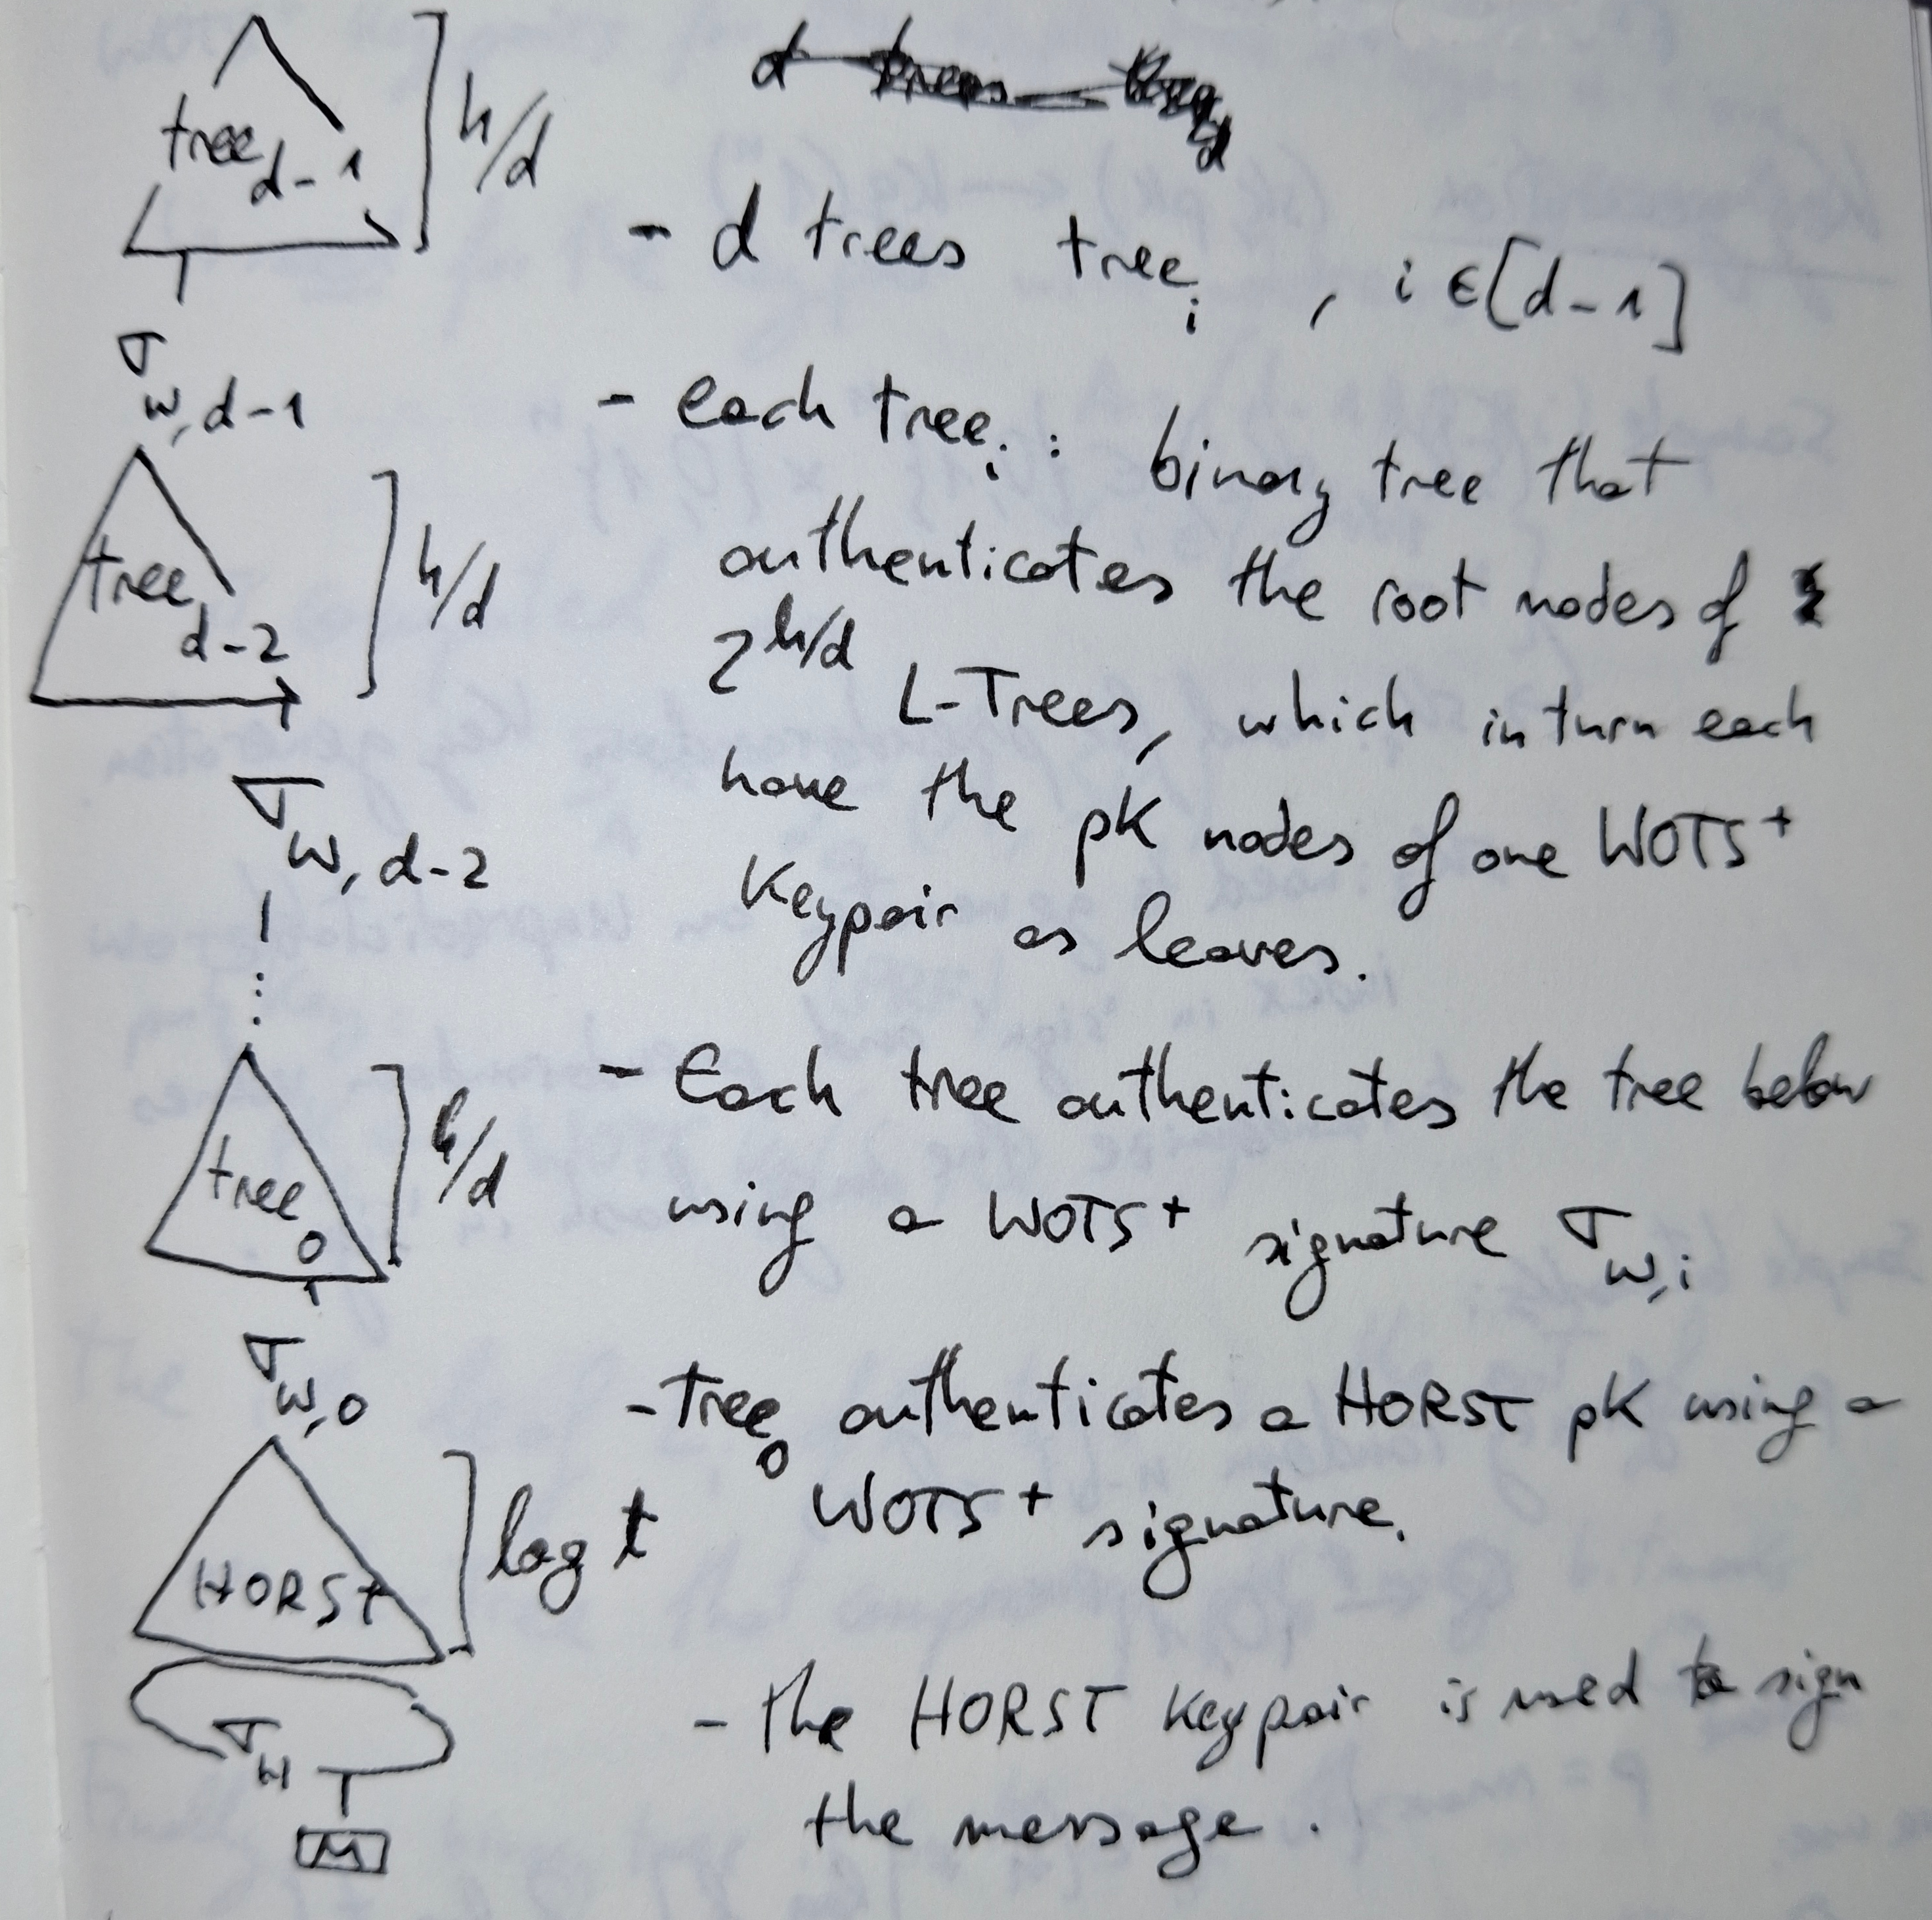
\includegraphics[width=0.9\textwidth]{img/sphincs-trees.jpg}
    % \caption{ }
    \label{fig:trees}
\end{figure}

An address is a bit string of length
$$a=\lceil
\underbrace{\log(d+1)}_{\text{WOTS+ keypair addr}}
\rceil +
\underbrace{(d-1)(h/d)}_{\stackrel{\text{index of the tree}}{\text{in the layer}}}
+
\underbrace{(h/d)}_{\stackrel{\text{index of the WOTS+}}{\text{key pair within the tree}}}
$$
$$= \lceil \log(d+1) \rceil + h$$

$\longrightarrow$ in SPHINCS-256, an address needs 64 bits.


\vspace{0.6cm}

\subsubsection{key generation:} $(sk, pk) \leftarrow keygen(1^n)$

sample $(sk_1, pk_1) \in \{0,1\}^n \times \{0,1\}^n$

$sk_1$: used for pseudorandom key generation

$sk_2$: used to generate an unpredictable index in 'sign' and pseudorandom values to randomize the msg hash in 'sign'.


Sample bitmasks: $p$ uniformly random n-bit values
$$Q \leftarrow^R \{0,1\}^{p \times n}$$

where $p = max \{ w-1, 2(h+ \lceil \log(l) \rceil), 2 \log t \}$.


We use
\begin{itemize}
    \item $Q_{WOTS+}$ for the fist $w-1$ bitmasks (of length $n$) in $Q$
    \item $Q_{HORST}$ for the first $2 \log t$
    \item $Q_{L-Tree}$ for the first $2 \lceil \log l \rceil$
    \item $Q_{Tree}$ for the $2h$ strings of length $n$ in $Q$ that follow $Q_{L-Tree}$
\end{itemize}

Remaining logic in keygeneration: generate the root node of the tree on layer $d-1$.



WOTS+R keypairs for the single tree at layer $d-1$ are generated\\
$\longrightarrow$ seed for the keypair with address $A=(d-1 || 0 || i)$ with $i \in [2^{h/d}-1]$ is computed as
$$S_A \leftarrow \mathcal{F}_a(A, sk_1)$$
where $\mathcal{F}$ is a PRF.


WOTS+ pub key:
$$pk_A \leftarrow WOTS.keygen(S_A, Q_{WOTS+})$$


The i-th leaf $L_i$ of the tree is the root of an L-Tree that compresses $pk_A$ using bitmasks $Q_{L-Tree}$.

Finally, a binary tree is build using the constructed leaves and its root node becomes $pk_1$.

\vspace{0.5cm}
SPHINCS $sk=(sk_1, sk_2, Q)$, $pk=(pk_1, Q)$.

\subsubsection{Signature algorithm} $\Sigma \leftarrow sign(M, sk)$

$M \in \{0,1\}^*$

Compute a randomized message digest $D \in \{0,1\}^m$:\\
compute pseudorandom $R=(R_1, R_2) \in \{0,1\}^n \times \{0,1\}^n$
$$R \leftarrow \mathcal{F}(M, sk_2)$$

then
$$D \leftarrow \mathcal{H}(R_1, M)$$
ie. randmized hash of $M$; where $R_1$ are the first $n$ bits of $R$.

$R_2$ (later $n$ bits of $R$) are used to select a HORST keypair:\\
compute an $h$ bit index $i \leftarrow CHOP(R_2, h)$ as the first $h$ bits of $R_2$.

Given index $i$, HORST key pair with address
$$A_{HORST} = (d || i(9,(d-1) h/d) || i ((d-1)h/d, h/d))$$
is used to sign the message digest $D$.\\
\hspace*{4em}ie. first $(d-1)h/d$ bits of $i$ are used as tree index and the remaining bits for the index within the tree.

The HORST signature and public key

$$(\sigma_H, pk_H) \leftarrow (D, S_{A_{HORST}}, Q_{HORST})$$
are computed using the HORST bitmasks and the seed
$$S_{A_{HORST}} \leftarrow \mathcal{F}_a(A_{HORST}, sk_1)$$

Signature:
$$\Sigma = (i, R_1, \sigma_H, \sigma_{W,0}, Auth_{A_0}, \sigma_{W,d-1}, Auth_{A_{d-1}})$$

where
\begin{itemize}
    \item[ ] $\sigma_H$: HORST signature
    \item[ ] $\sigmA_{W,0}$: WOTS+ signature
    \item[ ] $Auth_{A_0}$: one auth path per layer.
\end{itemize}

\subsubsection{Verification} $b \leftarrow vf(M, \Sigma, pk)$

compute message digest $D \leftarrow \mathcal{H}(R_1, M)$ ($R_1$ comes from $\Sigma$)

$$pk_H \leftarrow HORST.vf(D, \sigma_H, Q_{HORST})$$
where $Q_{HORST}$ comes from $pk$.

$$pk_{W,0} \leftarrow WOTS.vf(pk_H, \sigma_{W,0}, Q_{WOTS+})$$

where $\sigma_{W,0}$ is the WOTS+ signature, and $Q_{WOTS+}$ is the WOTS+ bitmask.

An L-Tree is used to compute $L_{i((-1)h/d, h/d)}$, ie. the leaf corresponding to $pk_{W,0}$.

Then, compute $Root_0$ with index $i((d-1)h/d, h/d)$, leaf $L_{i((d-1)h/d, h/d)}$ and authentication path $Auth_0$.

This procedure is repeated for layers $1$ to $d-1$ with the following differences:
\begin{enumerate}
    \item on layer $1 \leq j < d$, the root of the previous tree, $Root_{j-1}$, is used to compute the WOTS+ $pk_{w,j}$.

    \item the leaf from $pk_{w,j}$ using an L-Tree is $L_{i((d-1)h/d, h/d)}$; ie. the index of the leaf within the tree can be computed cutting off the last $j(h/d)$ bits of $i$ and then using the last $(h/d)$ bits of the resulting bit string.
\end{enumerate}

The result of the final repetition on layer $d-1$ is a value $Root_{d-1}$ (root of the single tree on the top layer).

Then verifier checks
$$pk_1 \stackrel{?}{=} Root_{d-1}$$

\subsubsection{Sizes of SPHINCS-256}
\begin{itemize}
    \item pk: 1056 bytes
    \item sk: 1088 bytes
    \item sig: 41000 bytes
\end{itemize}

\begin{figure}[H]
    \centering
    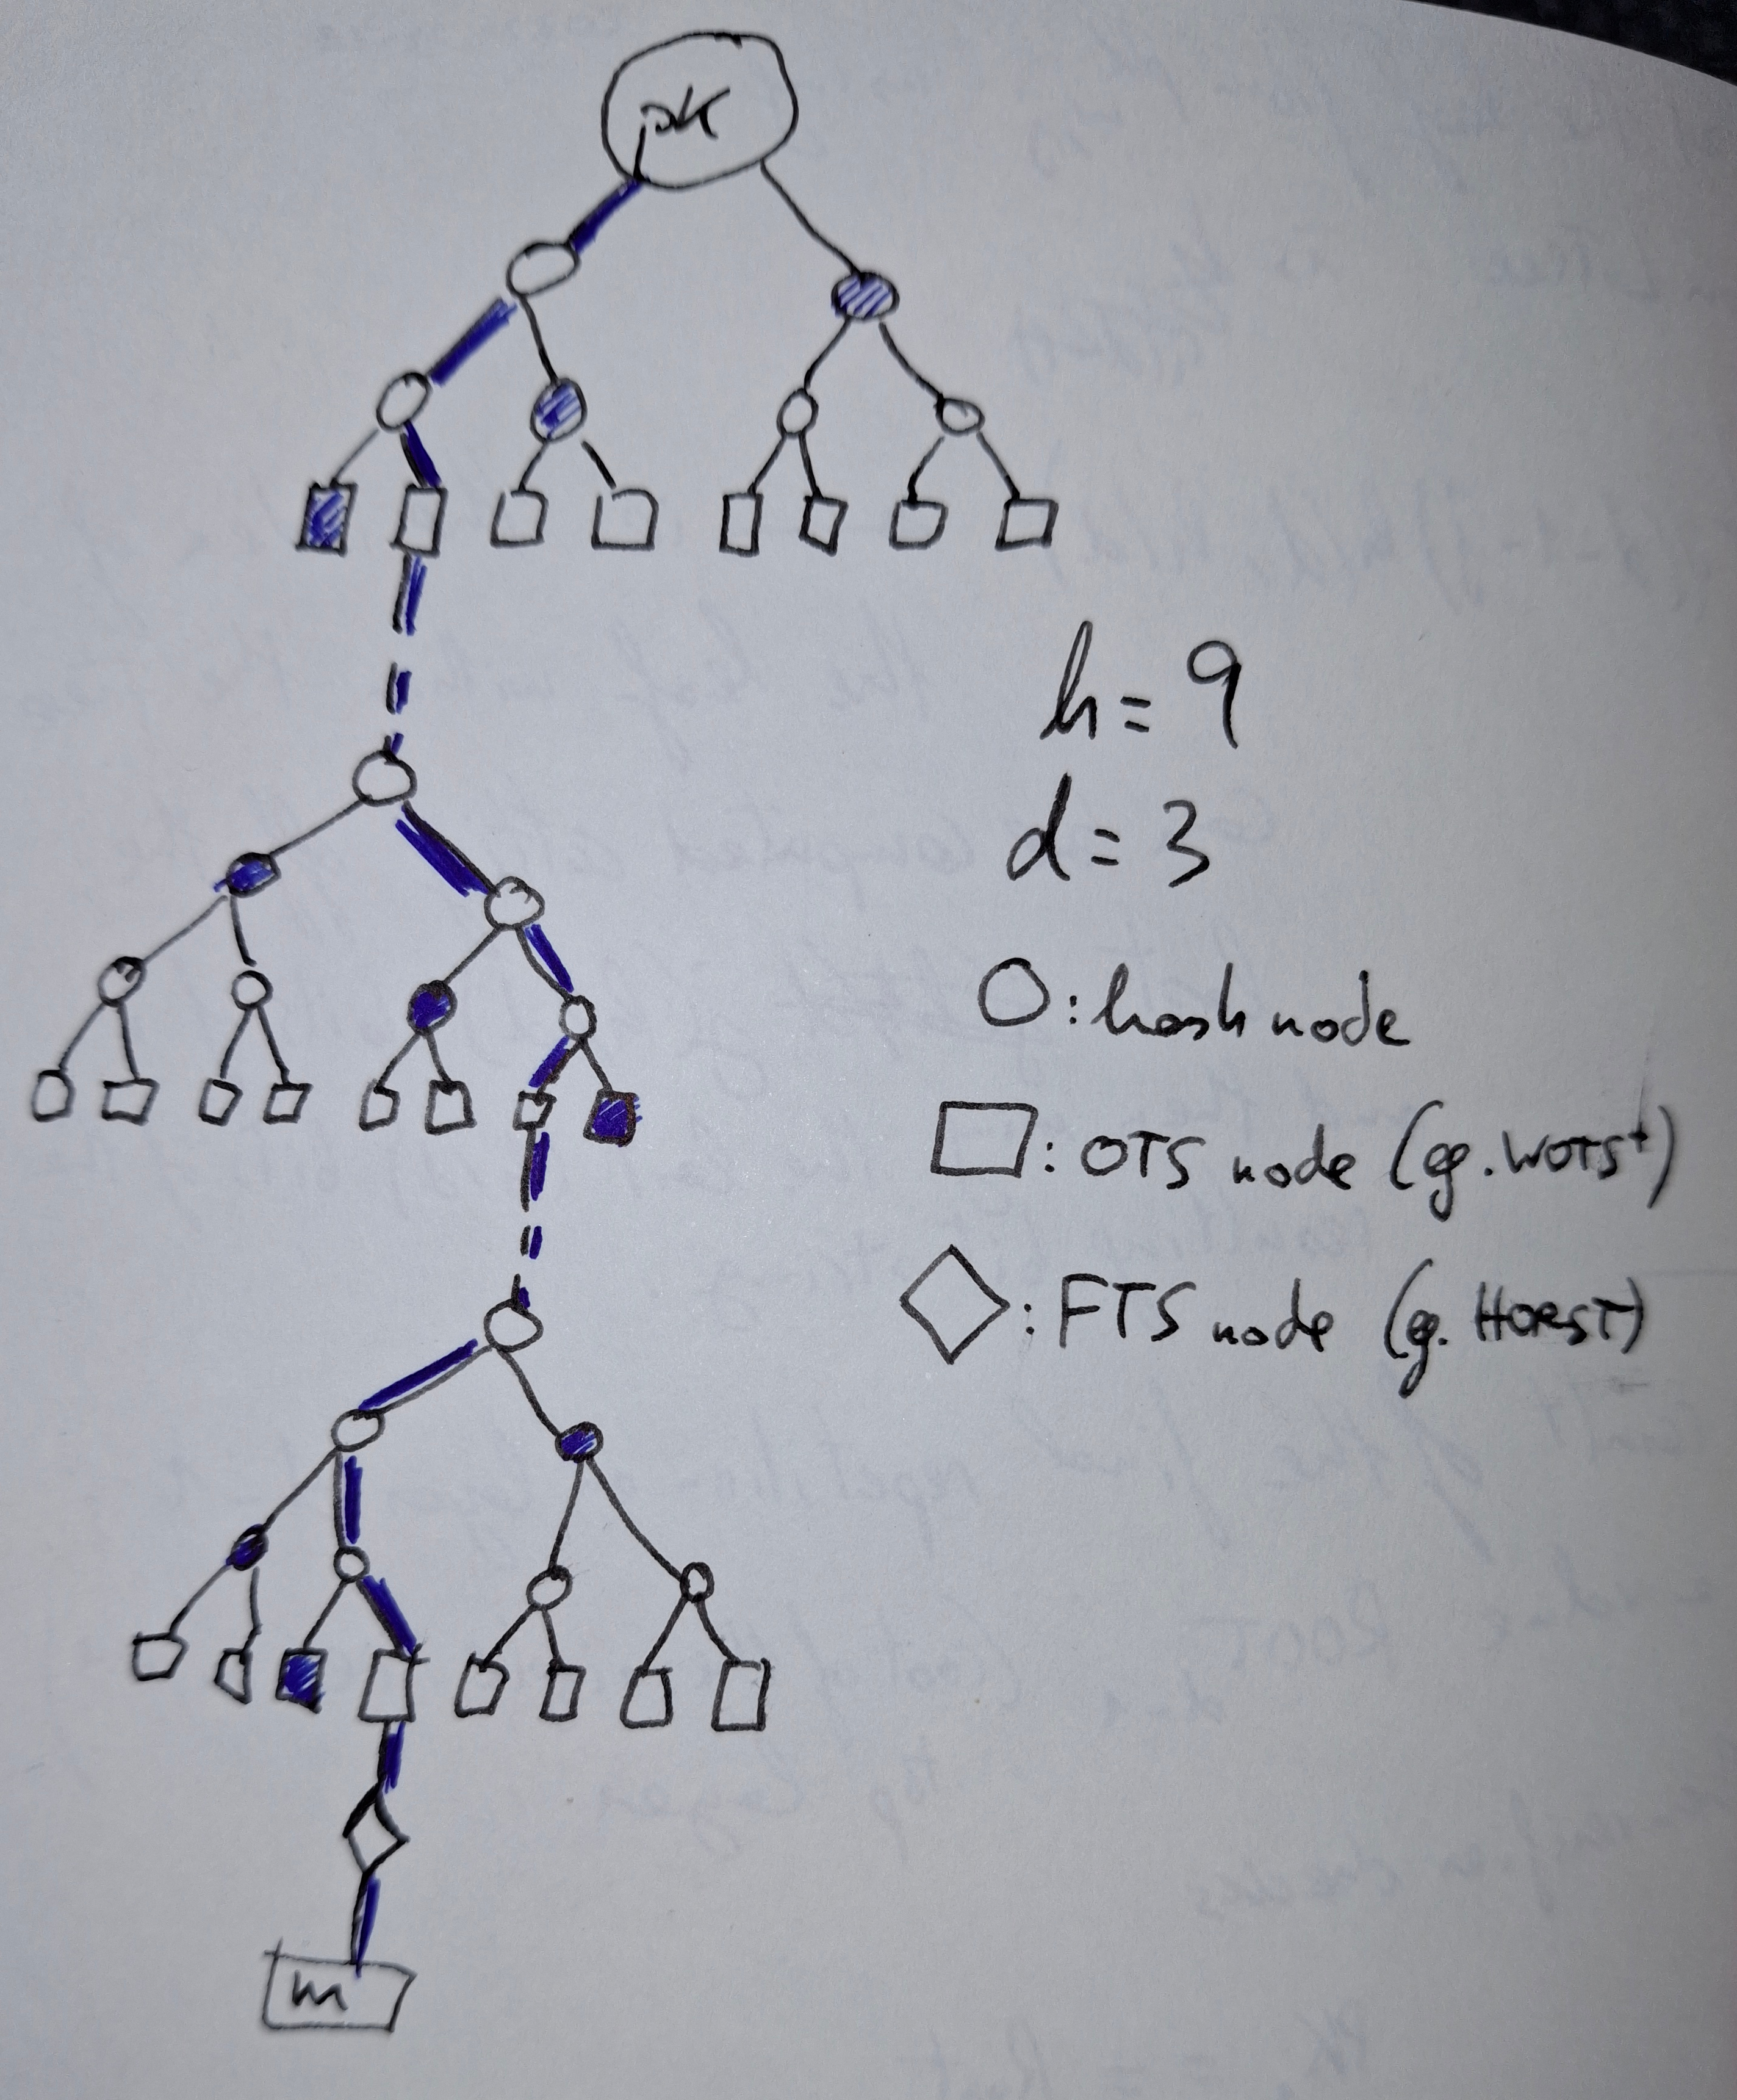
\includegraphics[width=0.9\textwidth]{img/sphincs-hyper-tree.jpg}
    % \caption{Hyper-Tree}
    \label{fig:hyper-tree}
\end{figure}

\section{XMSS (2011)}
After seeing the previous schemes of this document, XMSS signatures are quite straight forward:

MerkleTree which leaves are WOTS+ public keys. Each leaf has a corresponding
one-time key $(sk_i, pk_i)$

To sign message number $i$:
$$\sigma_i = (i, R, \sigma_{WOTS+, i}, AuthPath_i)$$

Verifier reconstructs $pk_i$ from the WOTS+ signature, and then follows the authentication path to obtain the root.

\vspace{0.6cm}
Important: Never use the same WOTS+ leaf more than once. Thus it is important to keep track of the used leaves. ie. keep a state.

\bibliographystyle{unsrt}
\bibliography{notes_hash-based-signatures.bib}

\end{document}
